\thispagestyle{fancy}
\chapter{Kravspecifikation}
I denne del af bachelor-forbedrelsesjournalen vil projektets foreløbige funktionelle krav blive gennemgået. Kravene, der her bliver gennemgået, skal ses som midlertidige udkast, da projektets mål ikke er endeligt fastlagt.
\\ \\
I projektets context diagram vil systems overordnede struktur blive beskrevet. \\
Foreløbig er intentionen at projektet opdeles i tre særskilte del:\\
\begin{enumerate}
	\item En dataopsamlings del, hvor data kan opsamles, organiseres og glemmes, så det kan anvendes af de øvrige dele af projektet
	\item En machine-lerning-del, hvor den indsamlede data processeres. Videre skal der i denne del være mulighed for at begrænse, hvilke dele af den indsamlede data, der processeres
	\item En form for SDK-del, der kan anvendes i software, hvor der er behov for håndbevægelsesgenkendelse	
\end{enumerate}

\section{Kontekstdiagram}
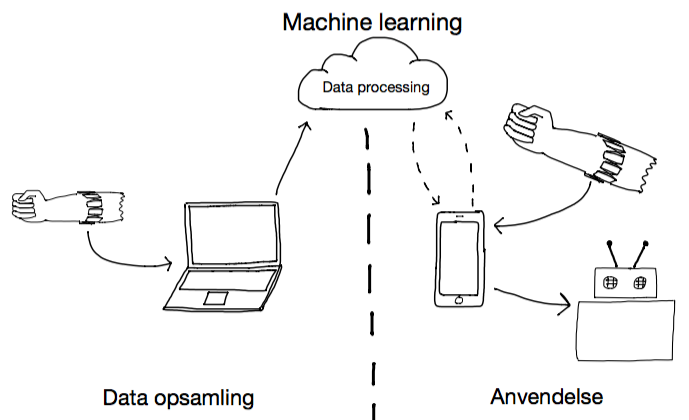
\includegraphics[width=1\textwidth]{kontekstdiagram}
\section{User case diagram}
Følgende use case diagram beskriver, projektets aktører i relation til de enkelte use cases, der foreløbigt er tiltænkt projektet.

\section{Aktørbeskrivelse}
\subsubsection*{Admin}
\subsubsection*{Testperson}
\subsubsection*{Udvikler}

\section{Fully dressed use cases}
I dette afsnit findes detaljerede beskrivelser af projektets use cases, dog er disse ikke fuldstændig gennemarbejdet, da stadig er en vis usikkerhed om projektets endelig.
\\ \\Særlig use case 5 og 6 er illustrative og beskriver den generelle idé om at genkendelse programmet bør kunne implementeres og anvendes i tredjeparts software.
\subsection{UC 1 - Indsaml datasæt}
\begin{table}[htbp] 
	\begin{tabular}{|p{5cm}|p{9cm}|}
		\hline
		\textbf{Navn} & Indsaml dataset \\ \hline
		\textbf{Use case ID} & U1 \\ \hline
		\textbf{initiering} & Admin initierer denne use case \\ \hline
		\textbf{Aktører} & Admin (Primær Aktør ) \\ & Testperson (Sekundær aktør) \\ \hline
		\textbf{samtigdige forekomster} & - \\ \hline
		\textbf{Prækondition} & Testperson har Myo båndet på og dataindsamlings software kører \\ \hline
		\textbf{Postkondition} & Data set er indsamlet \\ \hline
	\end{tabular}
\end{table}
\textbf{Hovedscenarie}
\begin{enumerate}
	\item Admin trykker på knap på at starte for at starte dataindsamlingen.
	\item Testpersonen laver håndtegn.
	\item Admin trykker på knap for at stoppe dataindsamlingen, når håndtegnsbevægelsen er slut.
	\item Admin vælger, hvilken bevægelsestype der er blevet indsamlet og angiver hvem testperson.
	\item Admin trykker på knap for at gemme datasættet.
\end{enumerate}

\subsection{UC 2 - Tilføj ny bevægelsestype}
\begin{table}[htbp] 
	\begin{tabular}{|p{5cm}|p{9cm}|}
		\hline
		\textbf{Navn} & Tilføj ny bevægelsestype \\ \hline
		\textbf{Use case ID} & U2 \\ \hline
		\textbf{initiering} & Admin initierer denne use case \\ \hline
		\textbf{Aktører} & Admin (Primær Aktør ) \\ \hline
		\textbf{samtigdige forekomster} & - \\ \hline
		\textbf{Prækondition} & Dataindsamlings softwaren kører \\ \hline
		\textbf{Postkondition} & En ny bevægelsestype er tilføjet til Dataindsamlings softwaren \\ \hline
	\end{tabular}
\end{table}
\textbf{Hovedscenarie}
\begin{enumerate}
	\item Admin trykker på knap for at tilføje ny bevægelsestype.
	\item Admin angiver title for den nye bevægelsestype.
	\item Admin tildeler evt. farve til den nye bevægelsestype.
	\item Admin vælger, hvilken bevægelsestype der er blevet indsamlet og angiver hvem testperson.
	\item Admin trykker på knap for at gemme bevægelsestypen.
\end{enumerate}

\subsection{UC 3 - Slet datasæt}
\begin{table}[htbp] 
	\begin{tabular}{|p{5cm}|p{9cm}|}
		\hline
		\textbf{Navn} & Slet datasæt \\ \hline
		\textbf{Use case ID} & U3 \\ \hline
		\textbf{initiering} & Admin initierer denne use case \\ \hline
		\textbf{Aktører} & Admin (Primær Aktør ) \\ \hline
		\textbf{samtigdige forekomster} & - \\ \hline
		\textbf{Prækondition} & Et datasæt skal eksistere \\ \hline
		\textbf{Postkondition} & Datasæt er slettet \\ \hline
	\end{tabular}
\end{table}
\textbf{Hovedscenarie}
\begin{enumerate}
	\item Admin vælger eksisterende datasæt.
	\item Admin trykker på knap for at slette valgte datasæt.
\end{enumerate}

\subsection{UC 4 - Verificering af ML genkendelse}
\begin{table}[htbp] 
	\begin{tabular}{|p{5cm}|p{9cm}|}
		\hline
		\textbf{Navn} & Verificering af ML genkendelse \\ \hline
		\textbf{Use case ID} & U4 \\ \hline
		\textbf{initiering} & Admin initierer denne use case \\ \hline
		\textbf{Aktører} & Admin (Primær Aktør ) \\ \hline
		\textbf{samtigdige forekomster} & - \\ \hline
		\textbf{Prækondition} & ML har kategoriseret bevægelse \\ \hline
		\textbf{Postkondition} & Admin har varificeret kategorisering  \\ \hline
	\end{tabular}
\end{table}
\textbf{Hovedscenarie}
\begin{enumerate}
	\item Admin tjekker ML kategoriseringer.
	\begin{enumerate}
		\item Korrekt kategorisering: admin verificerer kategorisering.
		\begin{enumerate}
			\item Verificering gemmes.
		\end{enumerate}
		\item Ukorrekt verificiering: admin ændre kategorisering.
		\begin{enumerate}
			\item Ny kategorisering gemmes som verificeret.
		\end{enumerate}
	\end{enumerate}
\end{enumerate}
\clearpage
\subsection{UC 5 - Anvendelse af bevægelsesgenkendelse}
\begin{table}[htbp] 
	\begin{tabular}{|p{5cm}|p{9cm}|}
		\hline
		\textbf{Navn} & Anvendelse af bevægelsesgenkendelse \\ \hline
		\textbf{Use case ID} & U5 \\ \hline
		\textbf{initiering} & Softwareudvikleren initierer denne use case \\ \hline
		\textbf{Aktører} & Softwareudvikleren (Primær Aktør ) \\ \hline
		\textbf{samtigdige forekomster} & - \\ \hline
		\textbf{Prækondition} & Softwareudvikleren har bevægelsesgenkendelses SDK\\ \hline
		\textbf{Postkondition} & Softwareudvikleren har anvendt bevægelsesgenkendelsen\\ \hline
	\end{tabular}
\end{table}
\textbf{Hovedscenarie}
\begin{enumerate}
	\item Softwareudvikleren implementerer SDK i egen software
	\item Softwareudvikleren anvender SDK til bevægelsesgenkendelse
\end{enumerate}

\subsection{UC 6 - Genkendelse af bevægelse}
\begin{table}[htbp] 
	\begin{tabular}{|p{5cm}|p{9cm}|}
		\hline
		\textbf{Navn} & Genkendelse af bevægelse  \\ \hline
		\textbf{Use case ID} & U6 \\ \hline
		\textbf{initiering} & Testpersonen initierer denne use case \\ \hline
		\textbf{Aktører} & Testperson (Primær Aktør )\\ & Softwareudvikler (Sekundær aktør) \\ \hline
		\textbf{samtigdige forekomster} & - \\ \hline
		\textbf{Prækondition} & Testperson har Myo bånd på, som er forbundet til softwareudviklerens software \\ \hline
		\textbf{Postkondition} & Håndbevægelse er blevet genkendt\\ \hline
	\end{tabular}
\end{table}
\textbf{Hovedscenarie}
\begin{enumerate}
	\item Testperson laver håndbevægelse
	\item Myo-data sendes til softwareudviklerens software på computer el.lign.
	\item Softwareudviklerens software processer Myo-data
	\item Myo-data genkendes
	\item Testpersonens håndbevægelse genkendes
\end{enumerate}